% VUT FIT MITAI
% MSZ 2021/2022
% Author: Vladimir Dusek
% Login: xdusek27

%%%%%%%%%%%%%%%%%%%%%%%%%%%%%%%%%%%%%%%%%%%%%%%%%%%%%%%%%%%%%%%%%%%%%%%%%%%%%%%%

% Path to figures
\graphicspath{{pds/peer_to_peer_site/figures}}

%%%%%%%%%%%%%%%%%%%%%%%%%%%%%%%%%%%%%%%%%%%%%%%%%%%%%%%%%%%%%%%%%%%%%%%%%%%%%%%%

\chapter{PDS~--~Sítě Peer-to-Peer: vlastnosti, chování, způsoby směrování. Strukturované a nestrukturované sítě.}

% Notes:

%%%%%%%%%%%%%%%%%%%%%%%%%%%%%%%%%%%%%%%%%%%%%%%%%%%%%%%%%%%%%%%%%%%%%%%%%%%%%%%%

\section{Zdroje}

\begin{compactitem}
    \item \path{08-p2p.pdf}
    \item \path{PDS_2021-04-09.mp4}
\end{compactitem}

%%%%%%%%%%%%%%%%%%%%%%%%%%%%%%%%%%%%%%%%%%%%%%%%%%%%%%%%%%%%%%%%%%%%%%%%%%%%%%%%

\section{Architektura peer-to-peer sítí}

\begin{compactitem}
    \item Peer-to-Peer (P2P) je alternativní architektura vůči client-server.
    \item Uzly (uživatelé) spolu komunikují napřímo. Každý uzel v síti má stejnou roli. Není zde žádný centrální bod, žádný uzel není nadřazený ostatním\footnote{Jsou výjimky.}.
    \item Jiný způsob adresování~--~adresování obsahem.
    \item Jiný způsob směrování~--~lokální rozhodování, specifická struktura sítí.
    \item Příklad: BitTorrent, Napster, Gnutella, Skype (dříve), Bitcoin, Bluetooth, instant messaging služby, \dots
\end{compactitem}

\paragraph*{Logická síť} Základem každé P2P sítě je tzv. logická síť (\textit{overlay}), která je vystavěna na aplikační vrstvě TCP/IP. Tedy P2P sítě staví nad exitující síťovou infrastrukturou. Logická síť definuje způsob propojení uzlů, směrování, vyhledávání informací, \dots

\paragraph*{Definice P2P sítě} Dynamický soubor nezávislých uzlů (peers), které jsou propojeny a jejichž zdroje (objekty) jsou k dispozici ostatním uzlům v této síti. Zdroje: výpočetní výkon, disková kapacita (soubory), zařízení (tiskárny). Sdílené zdroje jsou přímo přístupné všem uzlům, ty je nabízejí a zároveň využívají. Síť obsahuje prostředky pro připojení uzlu k síti, hledávání a využití zdrojů, \dots.

\paragraph*{Typy P2P sítí} \begin{compactitem}
    \item Pravé (pure)~--~Odebrání libovolného uzlu ze sítě nemá vliv na ztrátu schopnosti sítě poskytovat služby (např. Bitcoin).
    \item Hybridní~--~Pro svou činnost využívají centrální uzel pro poskytování části nabízených síťových služeb. Centrální bod slouží k autentizaci, indexování, inicializaci uzlu, apod.
\end{compactitem}

\paragraph*{Vlastnosti P2P sítí} \begin{compactitem}

    \item Samo-organizovatelnost: \begin{compactitem}
        \item Když se uzel připojí nebo odpojí, tak se síť přeskupí a funguje dále.
        \item Decentralizovaná topologie, kde uzly spolupracují na jejím vytvoření a udržování.
        \item Každý uzel je zodpovědný za svůj lokální stav a část informací (zdrojů).
        \item Uzly mají částečný pohled na topologii sítě (znají své nejbližší sousedy).
    \end{compactitem}

    \item Autonomní chování (samořiditelnost): \begin{compactitem}
        \item Uzly se chovají dle svého nejlepšího rozhodování (uzel pouze konzumuje zdroje, ale nechce poskytovat).
        \item Rozhodování je lokální a nepredikovatelné $\Rightarrow$ má vliv na topologii sítě, směrování, rozmístění objektů.
        \item Uzly se mohou chovat zlomyslně.
        \item Problém s ověřování identity uzlů a důvěryhodností (decentralizované řízení).
    \end{compactitem}

    \item Spolehlivost: \begin{compactitem}
        \item Spolehlivost sítě roste s redundancí uzlů a informací.
        \item Redundance objektů, kopie jsou umístěny ve více uzlech.
    \end{compactitem}

    \item Životnost uzlu: \begin{compactitem}
        \item Doba životnosti uzlu je neodhadnutelná $\Rightarrow$ problém s garancí služby.
        \item Závisí na subjektivním lokální rozhodnutí.
    \end{compactitem}

\end{compactitem}

\begin{figure}[H]
    \centering
    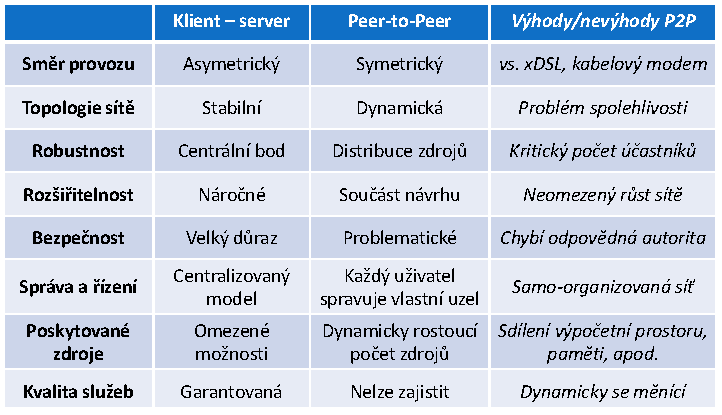
\includegraphics[width=0.9\linewidth]{p2p_vs_client_server.pdf}
    \caption{Srovnání vlastností P2P a klient-server architektur.}
\end{figure}

\paragraph*{Referenční model P2P} \begin{compactitem}
    \item Mějme množinu uzlů $P$, množinu zdrojů $R$ a množinu identifikátorů $I$.

    \item Struktura logické sítě: \begin{compactitem}
        \item mapování zdrojů: $F_R : R \rightarrow I$,
        \item mapování uzlů: $F_P : P \rightarrow I$.
        \item Množina uzlů $P$ zpřístupňuje zdroje $R$ v rámci jmenného prostoru $I$ pomocí $F_R$ a $F_P$.
    \end{compactitem}

    \item Decentralizovaná správa jmenného prostoru: \begin{compactitem}
        \item $M : I \rightarrow 2^P$
        \item Příklad: uzel potřebuje zjistit, kdo má konkrétní zdroj.
    \end{compactitem}

    \item Metrika blízkosti: \begin{compactitem}
        \item $d : I \times I \rightarrow \mathbb{R}$
        \item Příklad: uzel chce konkrétní zdroj, vyhledá všechny uzly, které ho poskytují a na základě metriky blízkosti vybere nejbližšího.
    \end{compactitem}
\end{compactitem}

\paragraph*{Geometrie sítě a směrování} \begin{compactitem}

    \item Geometrie (topologie). \begin{compactitem}
        \item Dynamická, uzly se připojují a odpojují.
        \item Množina uzlů $P$ zpřístupňuje zdroje $R$ v rámci jmenného prostoru $I$ pomocí $F_R$ a $F_P$.
    \end{compactitem}

    \item Směrování. \begin{compactitem}
        \item Každý uzel zná své sousedy (uzly a hrany k nim) pomocí relace sousedství: $N : P \rightarrow 2^P$ (uzel $\rightarrow$ jeho sousedi).
        \item Mějme předávání zprávy $route(p, m, i)$, kde hledáme cestu pro zprávu $m$, k uzlu $p$, který spravuje zdroj $i$. Směrování: kterému sousedovi mám zprávu předat?
        \item Distribuovaný proces nalezení cesty v síti P2P na základě lokálních znalostí.
        \item Směrovací funkce: $R : P \times I \rightarrow 2^P$.
        \item Směrovací tabulka: každý uzel má svoji, kterou si postupně plní a aktualizuje.
    \end{compactitem}

\end{compactitem}

%%%%%%%%%%%%%%%%%%%%%%%%%%%%%%%%%%%%%%%%%%%%%%%%%%%%%%%%%%%%%%%%%%%%%%%%%%%%%%%%

\section{Nestrukturované sítě}

\begin{compactitem}
    \item Neexistuje struktura uložení informace (zdroj (objekt) je umístěn na náhodném uzlu).
    \item Uzel si vyměňuje zprávy se svými sousedy (dotaz na vyhledávání konkrétního objektu).
    \item Když uzel hledá objekt, neví, jestli se přibližuje, dostává odpovědi pouze ano-ne.
    \item Jak v takovém systému směrovat (jak najít objekt skrze identifikátor)?
\end{compactitem}

\subsection{Záplava (\textit{flooding})} \begin{compactitem}
    \item Uzel pošle dotaz na objekt všem svým sousedům. \begin{compactitem}
        \item Pokud soused má objekt, pošle zpět odpověď.
        \item Pokud nemá, pošle zprávu svým sousedům.
    \end{compactitem}
    \item Lze omezit pomocí TTL ve zprávě (zamezuje zacyklení a zahlcení sítě).
\end{compactitem}

\begin{figure}[H]
    \centering
    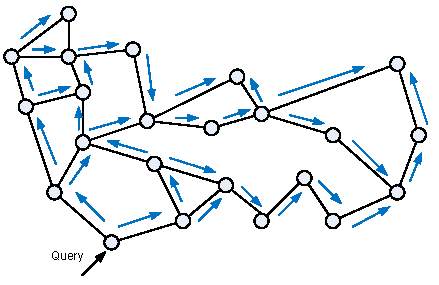
\includegraphics[width=0.6\linewidth]{flooding.pdf}
    \caption{Záplava.}
\end{figure}

\subsection{Rozšiřující se kruh (\textit{expanding ring})} \begin{compactitem}
    \item Uzel pošle dotaz na objekt všem svým sousedům s malým TTL. \begin{compactitem}
        \item Pokud objekt je nalezen, hledání končí.
        \item Pokud objekt není nalezen, zvýší se TTL a dotaz se pošle znovu.
    \end{compactitem}
    \item Redukuje počet zpráv v síti.
\end{compactitem}

\begin{figure}[H]
    \centering
    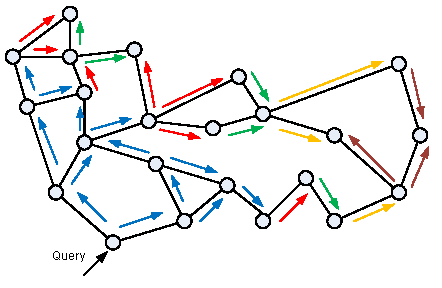
\includegraphics[width=0.6\linewidth]{expanding_ring.pdf}
    \caption{Rozšiřující se kruh.}
\end{figure}

\subsection{Náhodný průchod (\textit{random walk})} \begin{compactitem}
    \item Uzel pošle dotaz na objekt náhodně vybraným sousedům (i více zároveň).
\end{compactitem}

\begin{figure}[H]
    \centering
    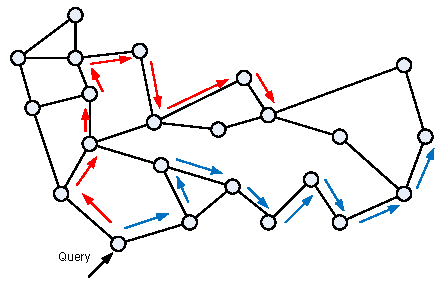
\includegraphics[width=0.6\linewidth]{random_walk.pdf}
    \caption{Náhodný průchod.}
\end{figure}

\subsection{Hledání lokálního minima (\textit{local minimum search})} \begin{compactitem}
    \item Není pro čistě nestrukturované sítě (přidává lokální vzdálenost).
    \item Máme množinu uzlů identifikovaných hodnotou $x$ a množinu objektů s identifikátorem $w$. Úkolem je umístit objekty do sítě uzlů tak, abychom je mohli najít rychle a spolehlivě, tj. jméno uzlu $x$ by mělo být co nejblíže jménu ukládaného objektu $w$.
    \item Při hledání používáme metriku vzdálenosti uzlu $x$ od objektu $w$~--~$d(x, w)$.
    \item Uzel $u$ je lokálním minimem pro objekt, pokud je jeho ID nejbližší k ID objektu mezi jeho sousedy do vzdálenosti $h$ kroků.
\end{compactitem}

\begin{figure}[H]
    \centering
    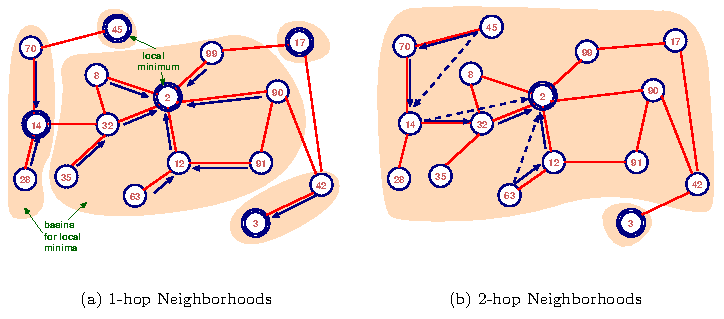
\includegraphics[width=1\linewidth]{lms.pdf}
    \caption{Příklad hledání lokálního minima. Uzly jsou značeny vzdáleností od objektu. $2-hop$~--~uzel zná sousedy sousedů a zapojuje je do hledání.}
\end{figure}

%%%%%%%%%%%%%%%%%%%%%%%%%%%%%%%%%%%%%%%%%%%%%%%%%%%%%%%%%%%%%%%%%%%%%%%%%%%%%%%%

\section{Strukturované sítě}

\begin{compactitem}
    \item Kombinují geometrické struktury a směrování.
    \item Distribuované směrovací algoritmy (metriky: shoda prefixu, euklidovská či lineární vzdálenost, XOR, \dots).
    \item Struktura sítě odpovídá uložení zdrojů.
    \item Jak směrovat?
\end{compactitem}

\subsection{Kademlia~--~Distribuovaná hašovací tabulka (DHT)}

\begin{compactitem}
    \item Identifikátory uzlů i souborů jsou hash.
    \item Metrika blízkosti: bitový XOR ($d(a, b) = a \oplus b$).
    \item Pro směrování používá distribuovanou hašovací tabulku (DHT), která obsahuje informace o dalších uzlech a souborech. \begin{compactitem}
        \item Myšlenka: znám dobře svoje okolí, čím dále jsem, tím méně znám. Ale mám tam kontakty, kterých se můžu ptát a které mají lepší lokální informace.
        \item Každý uzel má uloženou DHT ze své perspektivy.
    \end{compactitem}
\end{compactitem}

\begin{figure}[htb!]
    \centering
    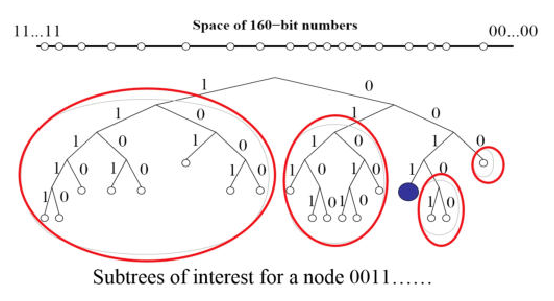
\includegraphics[width=1\linewidth]{dht_1.pdf}
    \caption{DHT se 160 bitovým jmenným prostorem. Uzly jsou umístěny ve stromu podle prefixů.}
\end{figure}

\begin{figure}[htb!]
    \centering
    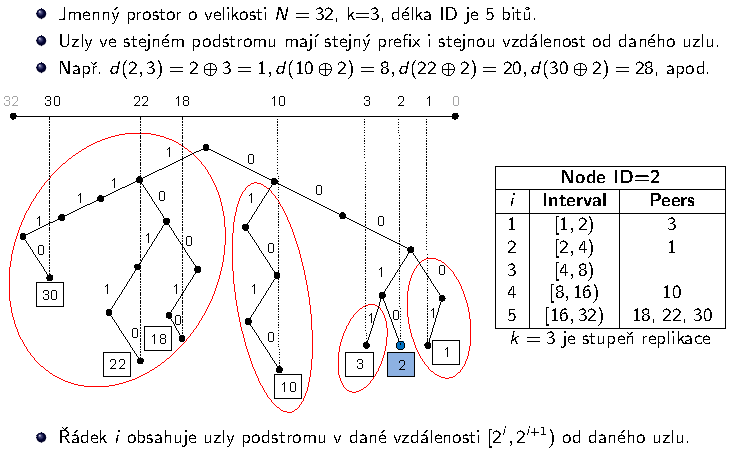
\includegraphics[width=1\linewidth]{dht_2.pdf}
    \caption{Konkrétní příklad DHT pro 5 bitový jmenný prostor. Napravo je směrovací tabulka uzlu 2. \textit{Interval} je interval vzdáleností a \textit{Peers} uzly co se v této vzdálenosti vyskytují.}
\end{figure}

\begin{compactitem}
    \item \textbf{Směrovací tabulka} vzniká dynamicky, tím že přijde zpráva od jiného uzlu (spočítá se vzdálenost a uzel se přidá do tabulky). \begin{compactitem}
        \item Pokud daný řádek obsahuje méně než k položek (počet replikací), tak se uzel přidá.
        \item Pokud je plný, tak zkontroluji, jestli jsou uzly dostupné, případně aktualizuju.
    \end{compactitem}
\end{compactitem}

\begin{figure}[htb!]
    \centering
    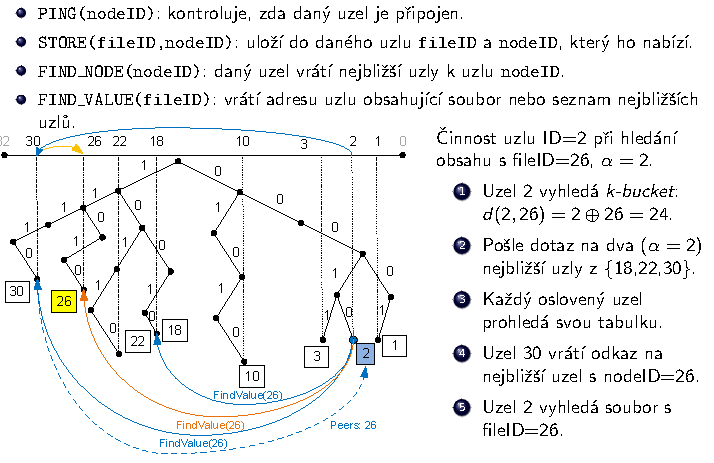
\includegraphics[width=1\linewidth]{dht_3.pdf}
    \caption{Příklad vyhledávání v DHT. Uzel $2$ hledá zdroj $26$. XOR vzdálenost $2$ a $26$ je $24$. Proto se ptá uzlů, které má ve vzdálenosti $\langle 16,32 )$. Jeden uzlů, podá přesnější informaci (uzel s ID 26). Uzel 2 se následně zeptá uzlu 26.}
\end{figure}

\begin{compactitem}
    \item Tento princip využívá P2P síť \textbf{BitTorrent} (buď využívá DHT a nebo koncept \textit{trackers}). \begin{compactitem}
        \item \textit{tracker}~--~Uzel, který má informace o tom, který uzel obsahuje jaké zdroje.
        \item \textit{torrent}~--~Soubor s informaci o sdílených souborech a s odkazem na tracker.
        \item BitTorrent je pak aplikační protokol pro distribuci souborů nad TCP.
    \end{compactitem}
\end{compactitem}
